\documentclass[12pt,a4paper]{article}
\usepackage[utf8]{vietnam}
\usepackage{amsmath,amssymb,tikz,tkz-tab}
\begin{document}
\section*{DẠNG 1: CỰC TRỊ CỦA HÀM SỐ $y=|f(x)|$ VÀ $y=|f(|x|)|$}
\cau1 Cho hàm số $f(x)$ có bảng biến thiên như sau:
\begin{center}
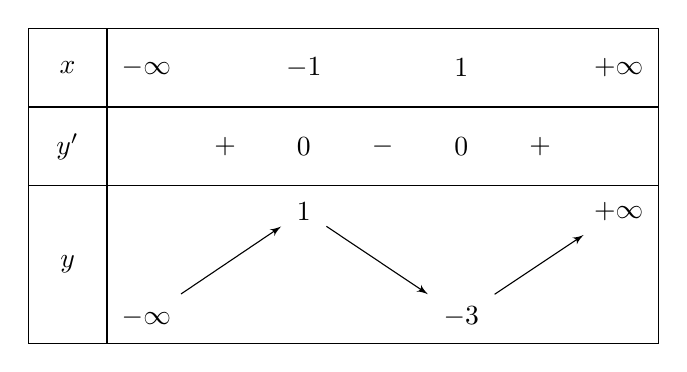
\begin{tikzpicture}
\tkzTabInit[nocadre=false,lgt=1,espcl=2]{$x$ /1,$y'$ /1,$y$ /2}{$-\infty$,$-1$,$1$,$+\infty$}
\tkzTabLine{,+,$0$,-,$0$,+,}
\tkzTabVar{-/$-\infty$,+/$1$,-/$-3$,+/$+\infty$}
\end{tikzpicture}
\end{center}
Hàm số $y=|f(x)|$ có bao nhiêu điểm cực trị?
\bonpa{2.}{3.}{5.}{4.}

\cau2 Cho hàm số $f(x)=-x^3+bx^2+cx+2$ với $b,c\in\mathbb{R}$. Biết rằng phương trình $f(x)=0$ có ba nghiệm dương phân biệt. Số điểm cực trị của hàm số $y=|f(|x|)|$ là
\bonpa{9.}{5.}{7.}{11.}
\section*{DẠNG 2: CỰC TRỊ CỦA HÀM SỐ $y=f(|x|)$}
\cau3 Cho hàm số $f(x)$ có đạo hàm $f'(x)=x(x-1)^2(x^2-4),\forall x\in\mathbb{R}$. Số điểm cực trị của hàm số $y=f(|x|)$ là
\bonpa{5.}{3.}{7.}{1.}
\end{document}
